\chapter{Half Wave Rectifier}
\vspace{-1cm}

%--------------------------AIM-----------------------------
\section{Aim}
\hspace{1cm}Single Phase Half Wave Uncontrolled and Controlled Rectifier

%--------------------------SOFTWARE USED-----------------------------
\section{Software Used}
\hspace{1cm}MATLAB R2020a
%-------------------------THEORY---------------------------
\section{Theory}
\hspace{\parindent}

A single phase half wave controlled rectifier circuit consists of an AC source, a thyristor, and a load. The thyristor conducts only when a gate pulse is applied to it, triggering it into the conducting state. The triggering angle (alpha) determines when the thyristor conducts, which allows the output voltage to be controlled. When the voltage across the thyristor becomes negative, it automatically turns off, and the circuit returns to a non-conducting state. This type of rectifier is widely used in applications that require precise control of the output voltage, such as in motor speed controllers and AC/DC converters.


% \vspace{1cm}

%----------------------Theoretical Calculations----------------------
\section{Theoretical Calculations}
\hspace{\parindent}
The theoretical calculations for a half-wave rectifier with an R load are given by the formulas:


$$
    V_{o,avg} =
    V_{phase}
    \sqrt{2(1 + cos\alpha)2\pi} =
    V_m(1 + cos\alpha)
    2\pi
$$
$$
    I_{o,avg} =
    V_oR
$$

In uncontrolled rectifiers, $ \alpha$ = 0, and the thyristor is replaced with a diode.
For a single-phase half-wave uncontrolled rectifier with an RMS voltage of 230V
and a resistive load of 10$ \Omega $,
the output voltage is 103.53V, and the output current is 10.53A.

For a single-phase half-wave controlled rectifier with an RMS voltage of 230V
and a resistive load of 10$ \Omega $ and a firing angle of $ \alpha  $ = 30◦, the output voltage
is 96.6V, and the output current is 9.66A.

\pagebreak

%-----------------------circuit 1--------------------------
\section{Single Phase Half Wave Uncontrolled Rectifier with R load}

\subsection{Circuit used for simulation}

% figure that is centered on the page
\begin{figure}[h]
    \centering
    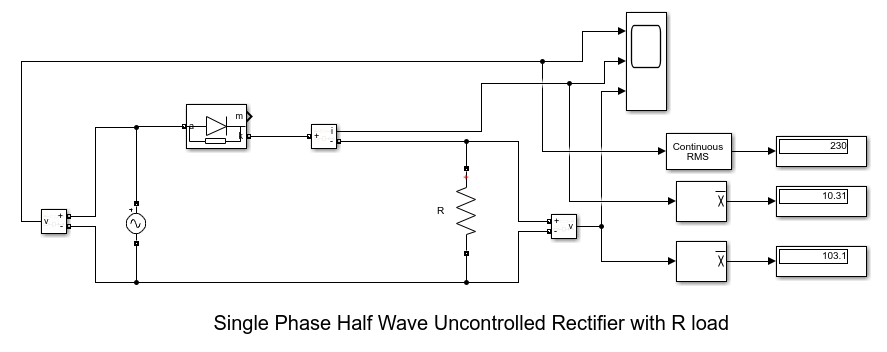
\includegraphics[width=0.7\textwidth]{images/experiment-1/circuit-diagram-simulation-01.png}
    \caption{Circuit used for simulation}
    \label{Fig_simulation_circuit_single-phase-half-wave-uncontrolled-rectifier-with-R-load}
\end{figure}

\subsection{Components Required}

\begin{table}[h]
    \renewcommand{\arraystretch}{1.3}
    \label{table_components_required_circuit_1}
    \centering
    \begin{tabular}{|c|c|c|c|}
        \hline
        Sr. No & Parameters                     & Ratings            & Quantity \\
        \hline
        \hline
        1      & AC Single Phase Voltage Source & 230V ($ V_{rms} $) & 1        \\
        \hline
        2      & Resistor                       & 10$ \Omega $       & 1        \\
        \hline
        3      & Diode                          & -                  & 1        \\
        \hline
        4      & Voltmeter                      & -                  & 2        \\
        \hline
        5      & Ammeter                        & -                  & 1        \\
        \hline
    \end{tabular}
    \caption{Components for Single Phase Half Wave Uncontrolled Rectifier with R load}

\end{table}




\subsection{Observations}

\begin{table}[h]
    \renewcommand{\arraystretch}{1.3}
    \label{table_observation_circuit_1}
    \centering
    \begin{tabular}{|c|c|c|}
        \hline
        Parameters                              & Theoretical Values & Simulation Values \\
        \hline
        \hline
        AC Input Voltage ($ V_{in,rms} $)       & 230V               & 230V              \\
        \hline
        Output Average Voltage ($ V_{o,avg} $)  & 103.53V            & 103.1V            \\
        \hline
        Output Average Current ($ I_{o,avg}  $) & 10.35A             & 10.31A            \\
        \hline
        AC Input Power ($ P_{AC}  $)            & 2389.5 W           & 2372 W            \\
        \hline
        DC Input Power ($ P_{DC}  $)            & 1071.53 W          & 1063 W            \\
        \hline
        Efficiency (\%)                         & 44.84              & 44.84             \\
        \hline
    \end{tabular}
    \caption{Observations for Single Phase Half Wave Uncontrolled Rectifier with R load}

\end{table}


The simulated values closely match the theoretical values, suggesting that the circuit is functioning correctly. Since the load is resistive, the output current is in phase with the output voltage. The output voltage and current waveforms indicate that the diode is forward-biased during the positive half-cycle of the AC source.

\pagebreak

\subsection{Resultant Waveforms}

% figure that is centered on the page
\begin{figure}[h]
    \centering
    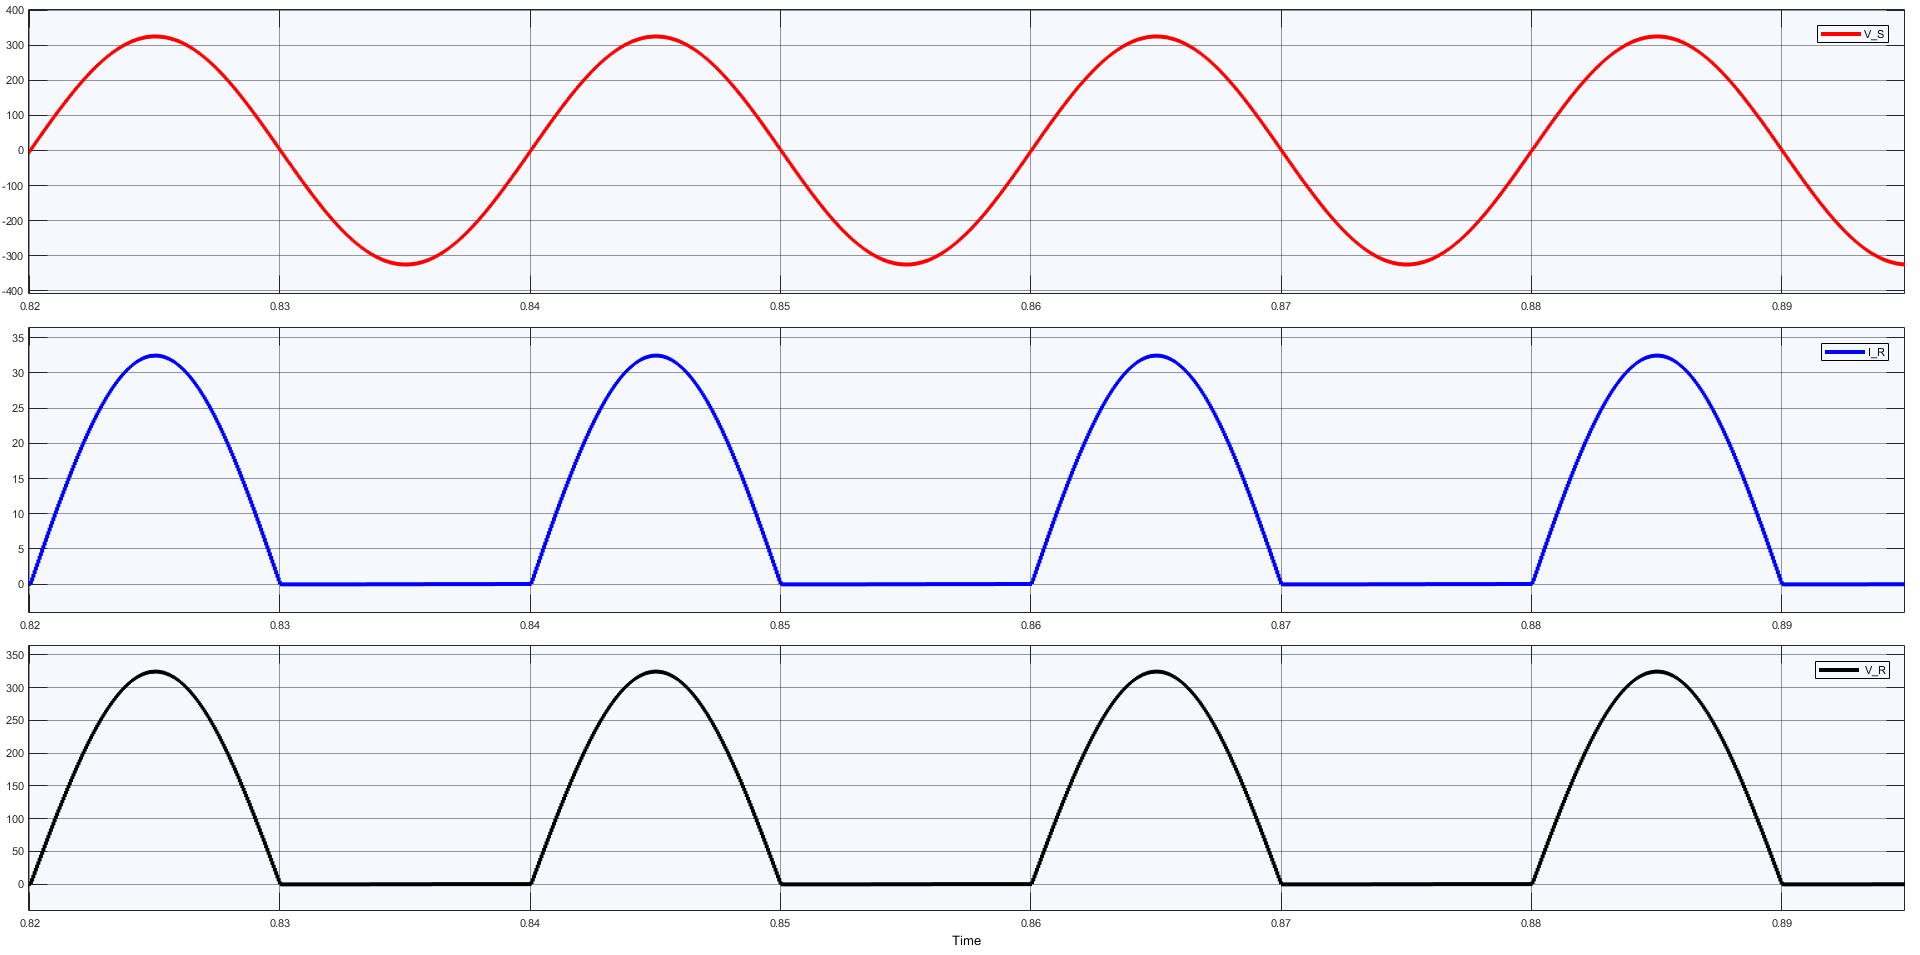
\includegraphics[width=1\textwidth]{images/experiment-1/circuit-scope-simulation-01.png}
    \caption{Scope Waveforms for Single Phase Half Wave Uncontrolled Rectifier with R load waveforms}
    \label{Fig_waveform_single-phase-half-wave-uncontrolled-rectifier-with-R-load}
\end{figure}

\pagebreak

%-----------------------circuit 2--------------------------
\section{Single Phase Half Wave Uncontrolled Rectifier with RL load}

\subsection{Circuit used for simulation}

% figure that is centered on the page
\begin{figure}[h]
    \centering
    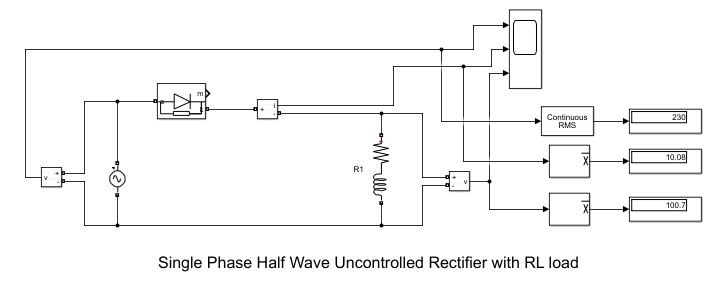
\includegraphics[width=0.7\textwidth]{images/experiment-1/circuit-diagram-simulation-02.png}
    \caption{Circuit used for simulation}
    \label{Fig_simulation_circuit_single-phase-half-wave-uncontrolled-rectifier-with-RL-load}
\end{figure}

\subsection{Components Required}

\begin{table}[h]
    \renewcommand{\arraystretch}{1.3}
    \label{table_components_required_circuit_2}
    \centering
    \begin{tabular}{|c|c|c|c|}
        \hline
        Sr. No & Parameters                     & Ratings            & Quantity \\
        \hline
        \hline
        1      & AC Single Phase Voltage Source & 230V ($ V_{rms} $) & 1        \\
        \hline
        2      & Resistor                       & 10$ \Omega $       & 1        \\
        \hline
        3      & Inductor                       & 10mH               & 1        \\
        \hline
        4      & Diode                          & -                  & 1        \\
        \hline
        5      & Voltmeter                      & -                  & 2        \\
        \hline
        6      & Ammeter                        & -                  & 1        \\
        \hline
    \end{tabular}
    \caption{Components for Single Phase Half Wave Uncontrolled Rectifier with RL load}
\end{table}


\subsection{Observations}

\begin{table}[h]
    \renewcommand{\arraystretch}{1.3}
    \label{table_observation_2}
    \centering
    \begin{tabular}{|c|c|c|}
        \hline
        Parameters                              & Theoretical Values & Simulation Values \\
        \hline
        \hline
        AC Input Voltage ($ V_{in,rms} $)       & 230V               & 230V              \\
        \hline
        Output Average Voltage ($ V_{o,avg} $)  & 103.53V            & 100.8V            \\
        \hline
        Output Average Current ($ I_{o,avg}  $) & 10.35A             & 10.08A            \\
        \hline
        AC Input Power ($ P_{AC} $)             & 2389.5 (W)         & 2318 (W)          \\
        \hline
        DC Input Power ($ P_{DC} $)             & 1071.53 (W)        & 1017 (W)          \\
        \hline
        Efficiency (\%)                         & 44.84              & 43.84             \\
        \hline
    \end{tabular}
    \caption{Observations for Single Phase Half Wave Uncontrolled Rectifier with RL load}

\end{table}


The circuit's simulated values are in good agreement with the theoretical values. Nonetheless, the load contains an inductive component that causes the output current to lag behind the output voltage. This delay results in the diode conducting until the output current reaches zero, which causes the output voltage to become negative during this period. Once the output current reaches zero, the diode stops conducting, and the output voltage returns to zero.
The efficiency of uncontrolled rectifier with RL load is 44.84\%.
\pagebreak


\subsection{Resultant Waveforms}

% figure that is centered on the page
\begin{figure}[h]
    \centering
    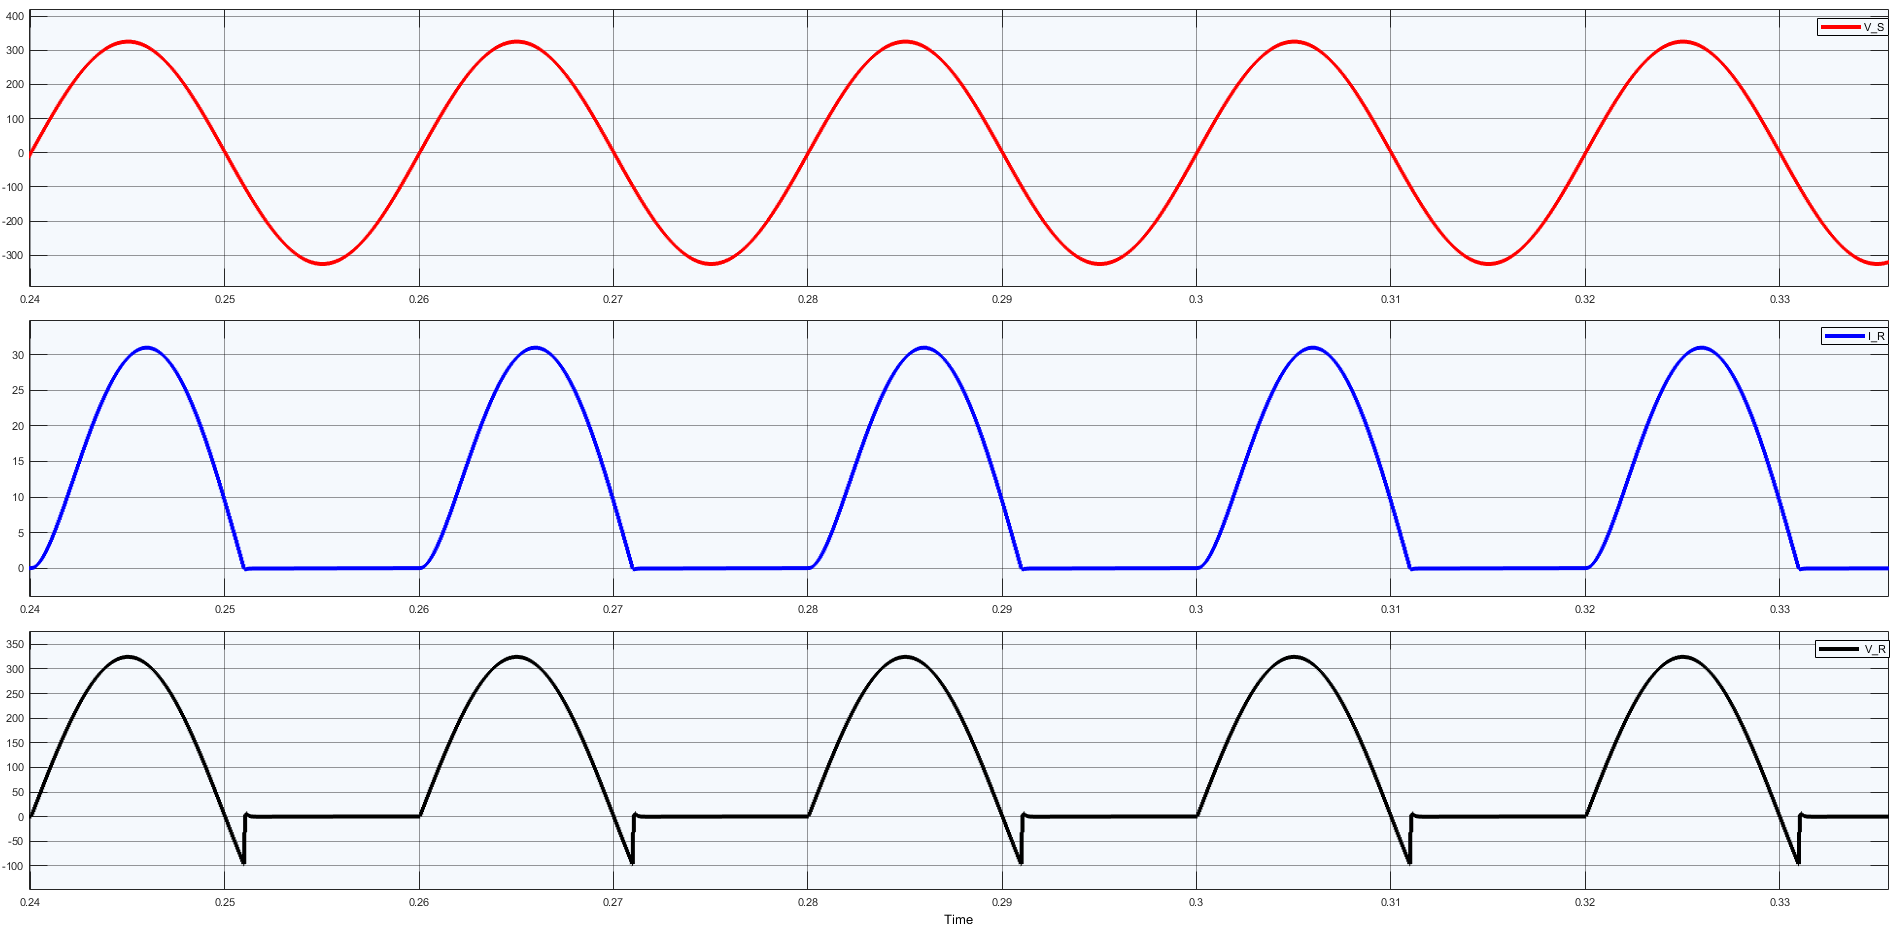
\includegraphics[width=1\textwidth]{images/experiment-1/circuit-scope-simulation-02.png}
    \caption{Scope Waveforms for Single Phase Half Wave Uncontrolled Rectifier with RL load}
    \label{Fig_waveform_single-phase-half-wave-uncontrolled-rectifier-with-RL-load}
\end{figure}

\pagebreak

\section{Single Phase Half Wave Uncontrolled Rectifier with RL load and Freewheeling Diode}

\subsection{Circuit used for simulation}

% figure that is centered on the page
\begin{figure}[h]
    \centering
    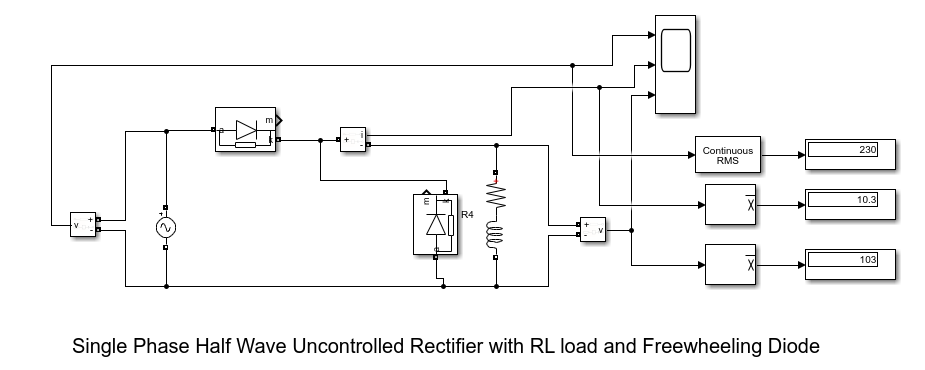
\includegraphics[width=0.7\textwidth]{images/experiment-1/circuit-diagram-simulation-03.png}
    \caption{Circuit used for simulation}
    \label{Fig_simulation_circuit_single-phase-half-wave-uncontrolled-rectifier-with-RL-load-and-freewheeling-diode}
\end{figure}

\subsection{Components Required}

\begin{table}[h]
    \renewcommand{\arraystretch}{1.3}
    \label{table_components_required_circuit_3}
    \centering
    \begin{tabular}{|c|c|c|c|}
        \hline
        Sr. No & Parameters                     & Ratings            & Quantity \\
        \hline
        \hline
        1      & AC Single Phase Voltage Source & 230V ($ V_{rms} $) & 1        \\
        \hline
        2      & Resistor                       & 10$ \Omega $       & 1        \\
        \hline
        3      & Inductor                       & 10mH               & 1        \\
        \hline
        4      & Diode                          & -                  & 1        \\
        \hline
        5      & Voltmeter                      & -                  & 2        \\
        \hline
        6      & Ammeter                        & -                  & 1        \\
        \hline
    \end{tabular}
    \caption{Components for Single Phase Half Wave Uncontrolled Rectifier with RL load and Freewheeling Diode}
\end{table}


\subsection{Observations}

\begin{table}[h]
    \renewcommand{\arraystretch}{1.3}
    \label{table_observation_3}
    \centering
    \begin{tabular}{|c|c|c|}
        \hline
        Parameters                              & Theoretical Values & Simulation Values \\
        \hline
        \hline
        AC Input Voltage ($ V_{in,rms} $)       & 230V               & 230V              \\
        \hline
        Output Average Voltage ($ V_{o,avg} $)  & 103.53V            & 103V              \\
        \hline
        Output Average Current ($ I_{o,avg}  $) & 10.35A             & 10.3A             \\
        \hline
        AC Input Power ($ P_{AC}  $)            & 2389.5 (W)         & 2404 (W)          \\
        \hline
        DC Input Power ($ P_{DC}  $)            & 1071.53 (W)        & 1061 (W)          \\
        \hline
        Efficiency (\%)                         & 44.84              & 44.13              \\
        \hline
    \end{tabular}
    \caption{Observations for Single Phase Half Wave Uncontrolled Rectifier with RL load and Freewheeling Diode}

\end{table}



The simulated and calculated values demonstrate that the simulated output voltage is close to the calculated voltage, but the simulated output current varies from the calculated current. Additionally, the inclusion of the freewheeling diode causes the output current in the rectifier circuit to cut off abruptly when the source AC supply reaches zero volts, as the lagging current begins to flow through the freewheeling diode rather than the rectifier circuit.
The efficiency of uncontrolled rectifier with RL load with freewheeling diode is 44.13\%.

\pagebreak

\subsection{Resultant Waveforms}


% figure that is centered on the page
\begin{figure}[h]
    \centering
    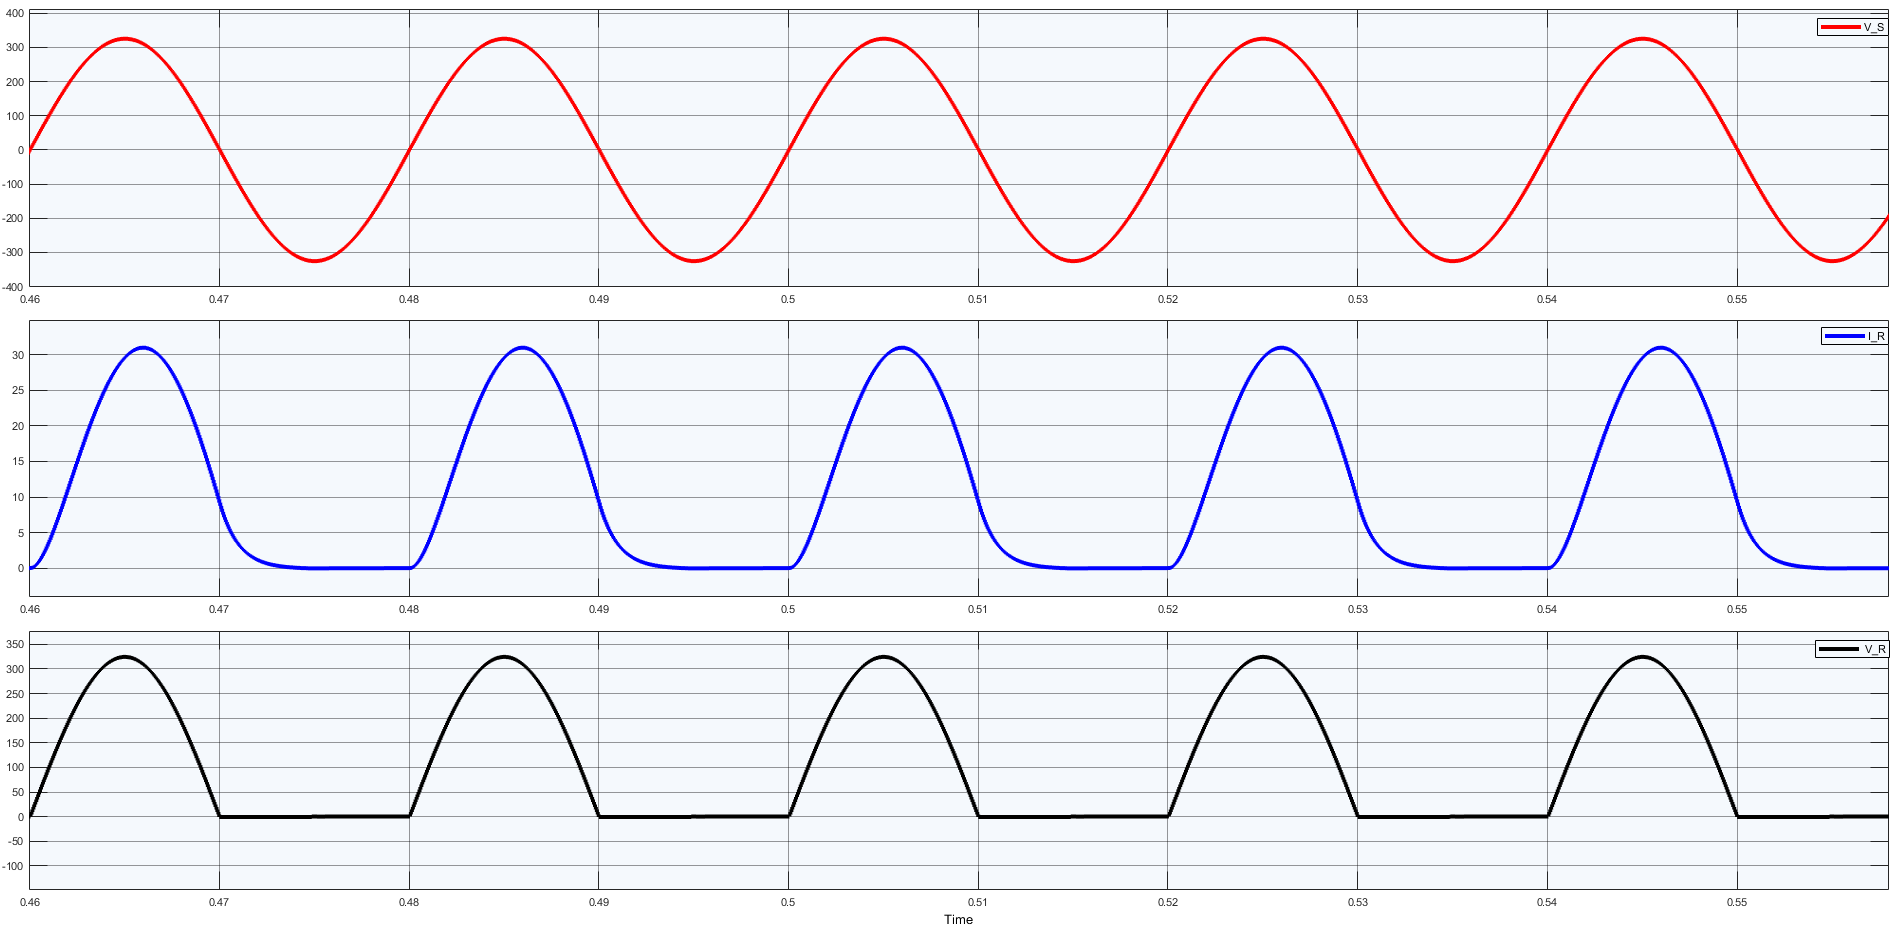
\includegraphics[width=1\textwidth]{images/experiment-1/circuit-scope-simulation-03.png}
    \caption{Scope Waveforms for Single Phase Half Wave Uncontrolled Rectifier with RL load and Freewheeling Diode}
    \label{Fig_waveform_single-phase-half-wave-uncontrolled-rectifier-with-RL-load-and-freewheeling-diode}
\end{figure}


\pagebreak


%-----------------------circuit 2--------------------------
\section{Single Phase Half Wave Uncontrolled Rectifier with RLE load}

\subsection{Circuit used for simulation}

% figure that is centered on the page
\begin{figure}[h]
    \centering
    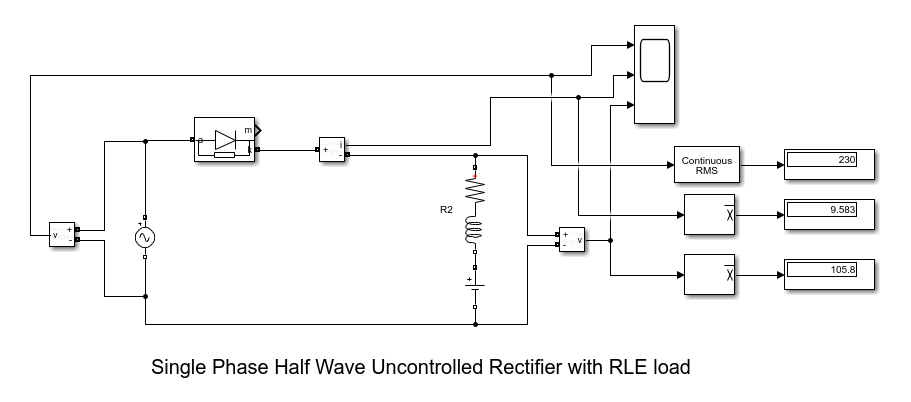
\includegraphics[width=0.7\textwidth]{images/experiment-1/circuit-diagram-simulation-04.png}
    \caption{Circuit used for simulation}
    \label{Fig_simulation_circuit_single-phase-half-wave-uncontrolled-rectifier-with-RLE-load}
\end{figure}

\subsection{Components Required}

\begin{table}[h]
    \renewcommand{\arraystretch}{1.3}
    \label{table_components_required_circuit_4}
    \centering
    \begin{tabular}{|c|c|c|c|}
        \hline
        Sr. No & Parameters                     & Ratings            & Quantity \\
        \hline
        \hline
        1      & AC Single Phase Voltage Source & 230V ($ V_{rms} $) & 1        \\
        \hline
        2      & Resistor                       & 10$ \Omega $       & 1        \\
        \hline
        3      & Inductor                       & 10mH               & 1        \\
        \hline
        4      & Diode                          & -                  & 1        \\
        \hline
        5      & DC Source                      & 100V               & 1        \\
        \hline
        6      & Voltmeter                      & -                  & 2        \\
        \hline
        7      & Ammeter                        & -                  & 1        \\
        \hline
    \end{tabular}
    \caption{Components for Single Phase Half Wave Uncontrolled Rectifier with RLE load}
\end{table}




\subsection{Observations}

\begin{table}[h]
    \renewcommand{\arraystretch}{1.3}

    \label{table_observation_4}
    \centering
    \begin{tabular}{|c|c|c|}
        \hline
        Parameters                              & Theoretical Values & Simulation Values \\
        \hline
        \hline
        AC Input Voltage ($ V_{in,rms} $)       & 230V               & 230V              \\
        \hline
        Output Average Voltage ($ V_{o,avg} $)  & 103.53V            & 105.8V            \\
        \hline
        Output Average Current ($ I_{o,avg}  $) & 10.35A             & 9.583A            \\
        \hline
        AC Input Power ($ P_{AC}  $)            & 2389.5 (W)         & 1290 (W)          \\
        \hline
        DC Input Power ($ P_{DC}  $)            & 1071.53 (W)        & 875.8 (W)         \\
        \hline
        Efficiency (\%)                         & 44.84              & 67.88             \\
        \hline
    \end{tabular}
    \caption{Observations for Single Phase Half Wave Uncontrolled Rectifier with RLE load}
\end{table}


The simulation results demonstrate that the output voltage waveform for the RL load has the same shape as the input voltage waveform but with a positive DC offset. This is due to the rectification process that converts the negative half cycle of the input waveform into a positive voltage. When the output current falls to zero, the diode stops conducting, and the output voltage becomes a constant 100V, which is equivalent to the peak value of the input AC voltage.
The efficiency of uncontrolled rectifier with RLE load is 67.88%.

\pagebreak

\subsection{Resultant Waveforms}

% figure that is centered on the page
\begin{figure}[h]
    \centering
    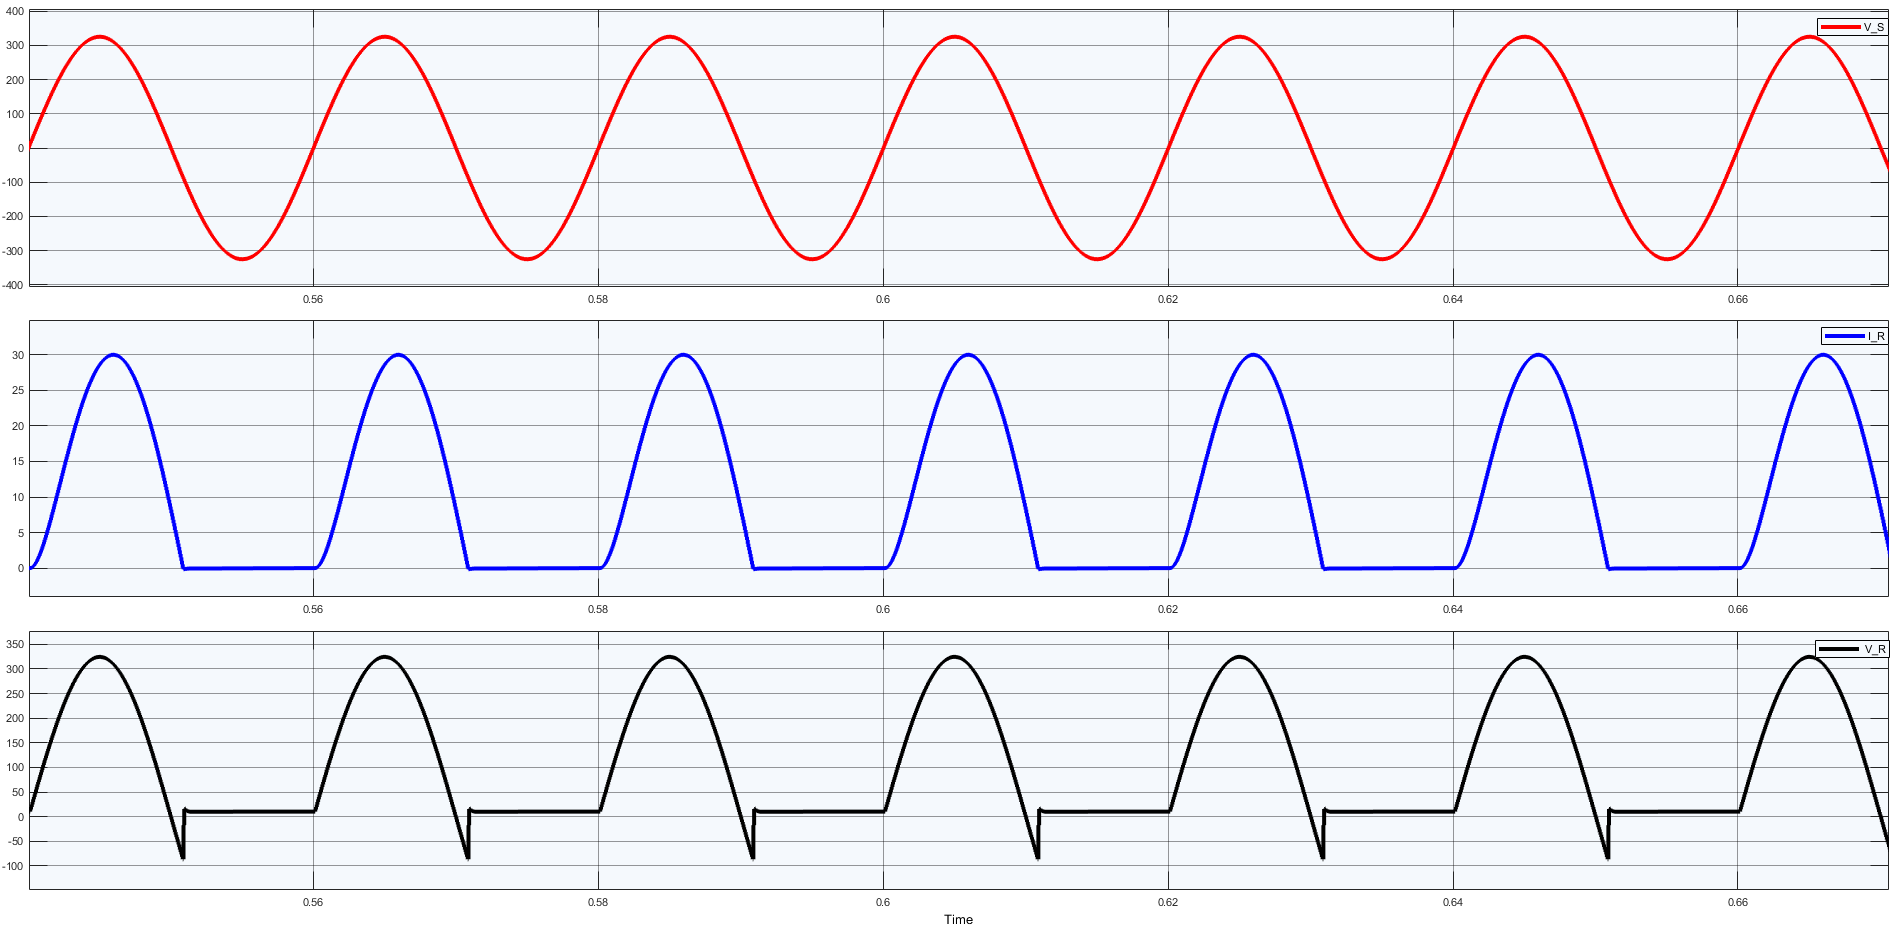
\includegraphics[width=1\textwidth]{images/experiment-1/circuit-scope-simulation-04.png}
    \caption{Scope Waveforms for Single Phase Half Wave Uncontrolled Rectifier with RLE load waveforms}
    \label{Fig_waveform_single-phase-half-wave-uncontrolled-rectifier-with-RLE-load}
\end{figure}

\pagebreak


\section{Single Phase Half Wave Controlled Rectifier with R load}

\subsection{Circuit used for simulation}

% figure that is centered on the page
\begin{figure}[h]
    \centering
    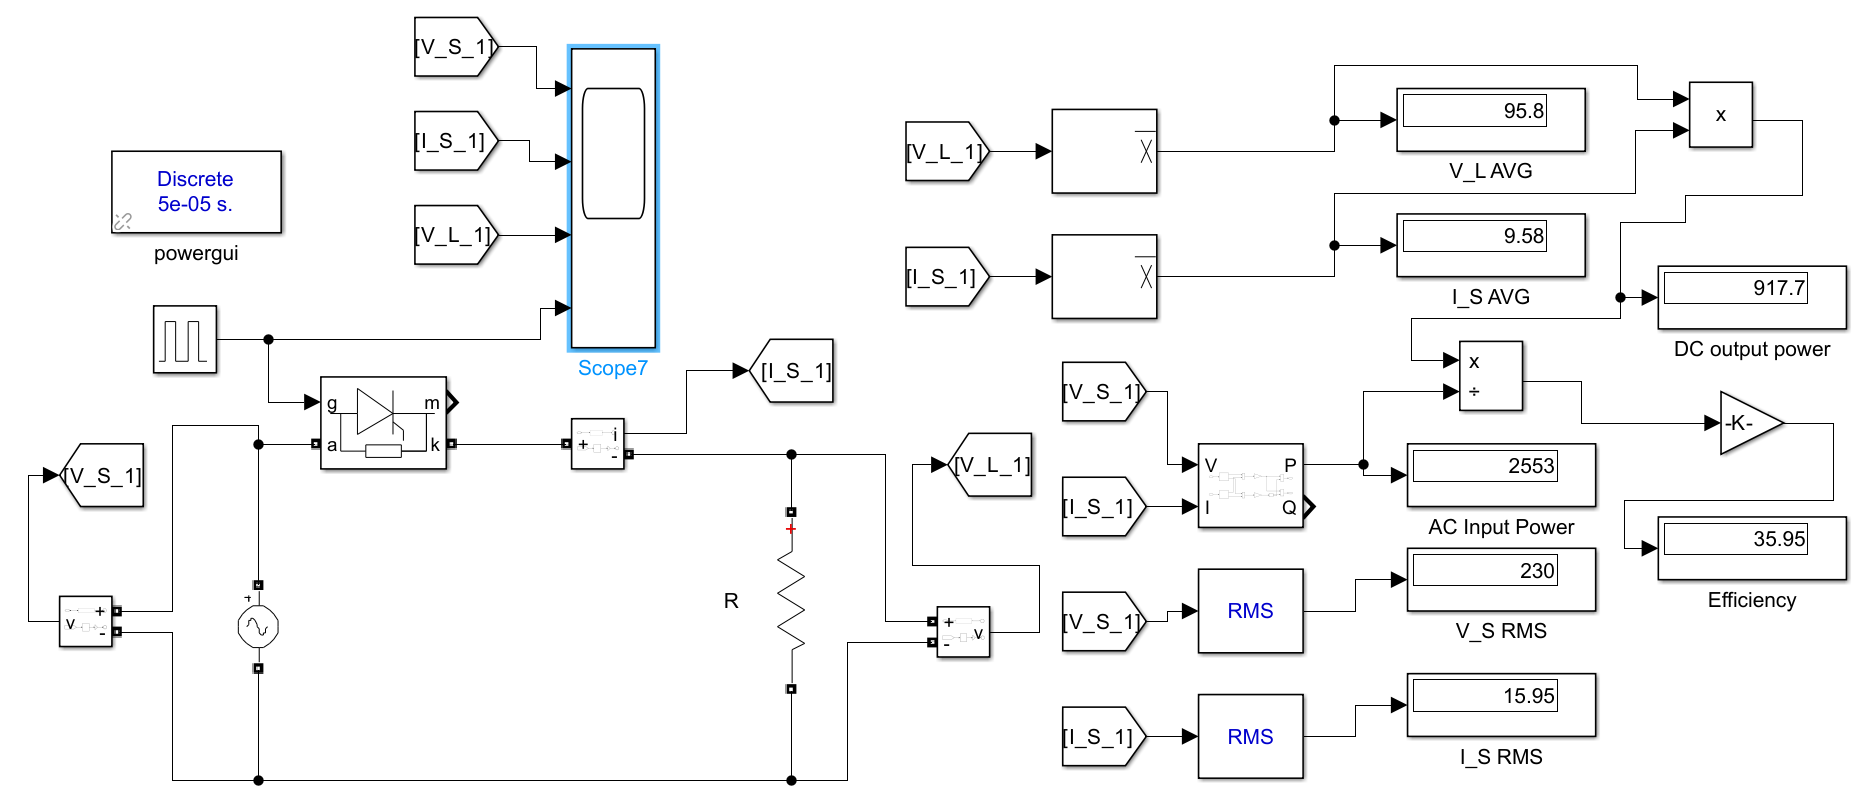
\includegraphics[width=1.0\textwidth]{images/experiment-1/circuit-diagram-experiment-05.png}
    \caption{Circuit for Single Phase Half Wave Controlled Rectifier with R load  (Firing Angle = 30$ ^\circ $)}
    \label{Fig_simulation_circuit_single-phase-half-wave-controlled-rectifier-with-R-load}
\end{figure}

\subsection{Components Required}

\begin{table}[h]
    \renewcommand{\arraystretch}{1.3}
    \label{table_components_required_single-phase-half-wave-controlled-rectifier-with-R-load}
    \centering
    \begin{tabular}{|c|c|c|c|}
        \hline
        Sr. No & Parameters                     & Ratings            & Quantity \\
        \hline
        \hline
        1      & AC Single Phase Voltage Source & 230V ($ V_{rms} $) & 1        \\
        \hline
        2      & Resistor                       & 10$ \Omega $       & 1        \\
        \hline
        3      & Inductor                       & 10mH               & 1        \\
        \hline
        4      & Diode                          & -                  & 1        \\
        \hline
        5      & Voltmeter                      & -                  & 2        \\
        \hline
        6      & Ammeter                        & -                  & 1        \\
        \hline
        7      & Thyristor                      & -                  & 1        \\
        \hline
    \end{tabular}
    \caption{Components for Single Phase Half Wave Controlled Rectifier with R load}

\end{table}



\subsection{Observations}

\begin{table}[h]
    \renewcommand{\arraystretch}{1.3}
    \label{table_observation_single-phase-half-wave-controlled-rectifier-with-R-load}
    \centering
    \begin{tabular}{|c|c|c|}
        \hline
        Parameters                              & Theoretical Values & Simulation Values \\
        \hline
        \hline
        AC Input Voltage ($ V_{in,rms} $)       & 230V               & 230V             \\
        \hline
        Output Average Voltage ($ V_{o,avg} $)  & 96.6V              & 95.8V            \\
        \hline
        Output Average Current ($ I_{o,avg}  $) & 9.66A              & 9.58A            \\
        \hline
        AC Input Power ($ P_{AC}  $)            & 2214.44 (W)        & 2553 (W)         \\
        \hline
        DC Input Power ($ P_{DC}  $)            & 926.98 (W)         & 917.7 (W)        \\
        \hline
        Efficiency (\%)                         & 41.86              & 35.95             \\
        \hline
    \end{tabular}
    \caption{Observations for Single Phase Half Wave Controlled Rectifier with R load}

\end{table}


The rectifier circuit is uncontrolled, and output voltage follows the shape of the input voltage. As the load is resistive in nature, the output current is in phase with the output voltage. The simulation results match the theoretical values reasonably well. However, the output voltage contains ripples due to the uncontrolled nature of the rectifier circuit.

The efficiency of controlled rectifier with R load is 35.95\%.

\pagebreak


\subsection{Resultant Waveforms}

% figure that is centered on the page
\begin{figure}[h]
    \centering
    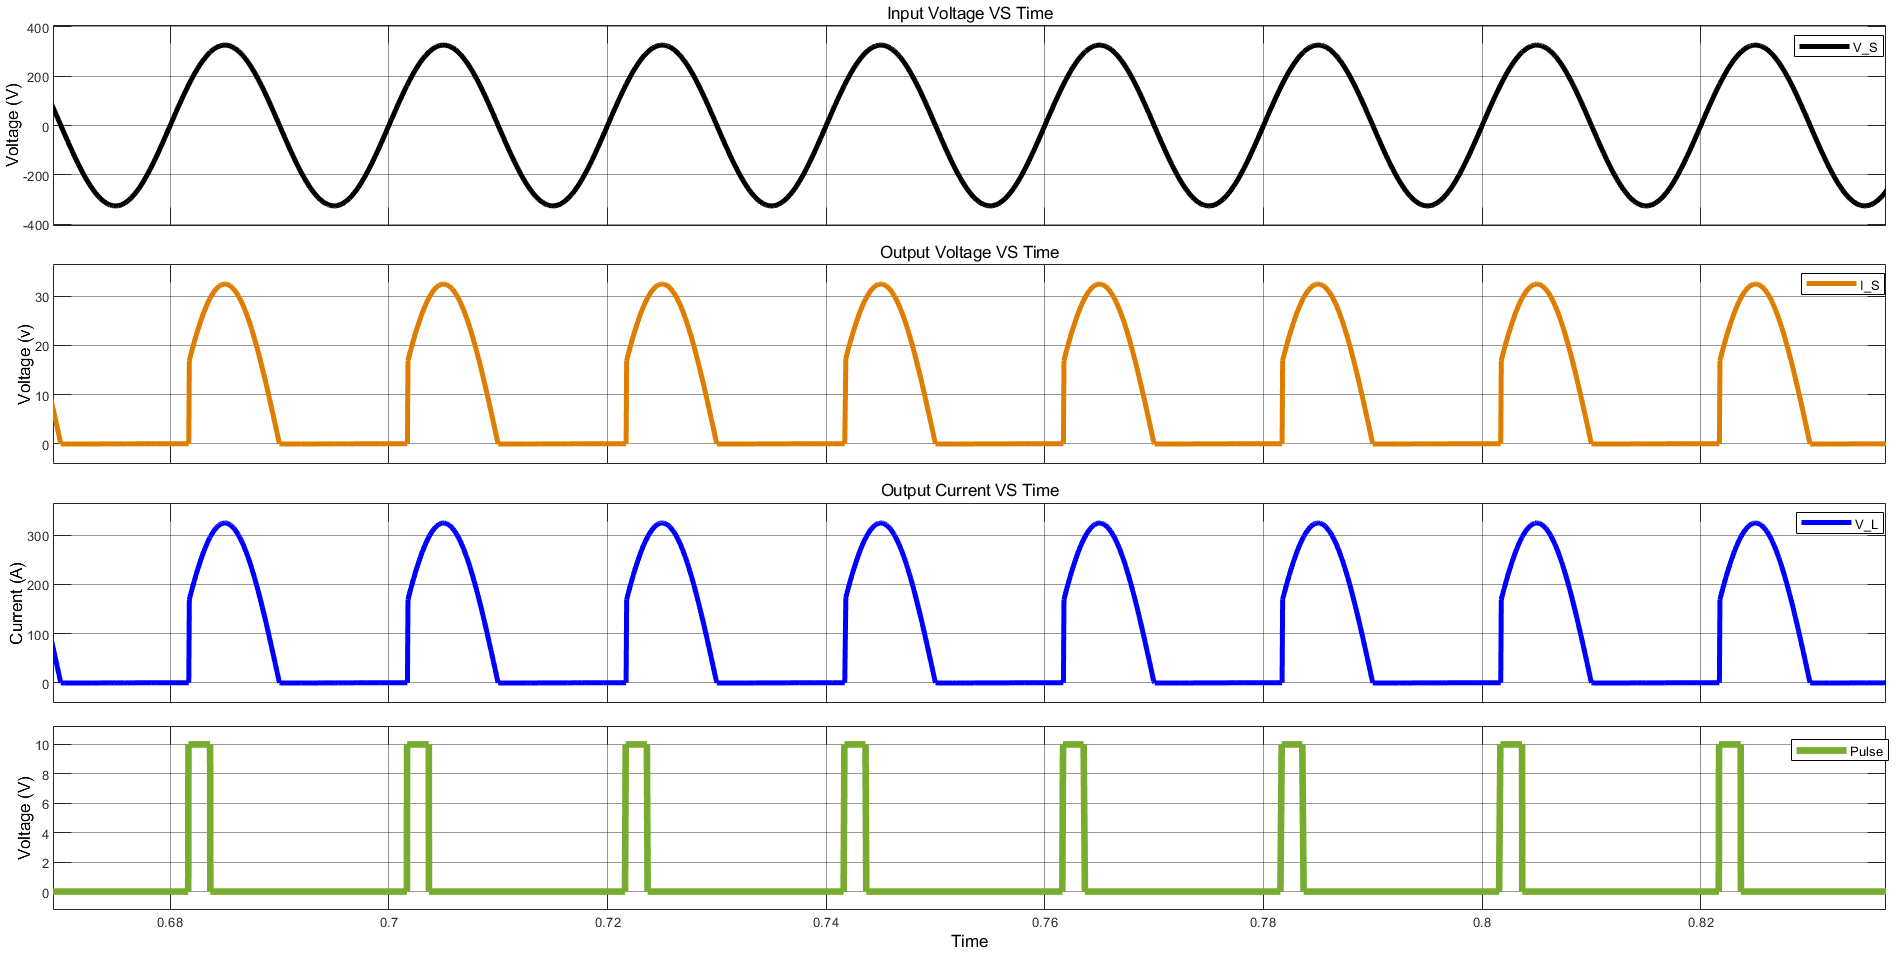
\includegraphics[width=1\textwidth]{images/experiment-1/circuit-scope-experiment-05.png}
    \caption{Scope Waveforms for Single Phase Half Wave Controlled Rectifier with R load}
    \label{Fig_waveform_single-phase-half-wave-controlled-rectifier-with-R-load}
\end{figure}

\pagebreak

\section{Single Phase Half Wave Controlled Rectifier with RL load}

\subsection{Circuit used for simulation}

% figure that is centered on the page
\begin{figure}[h]
    \centering
    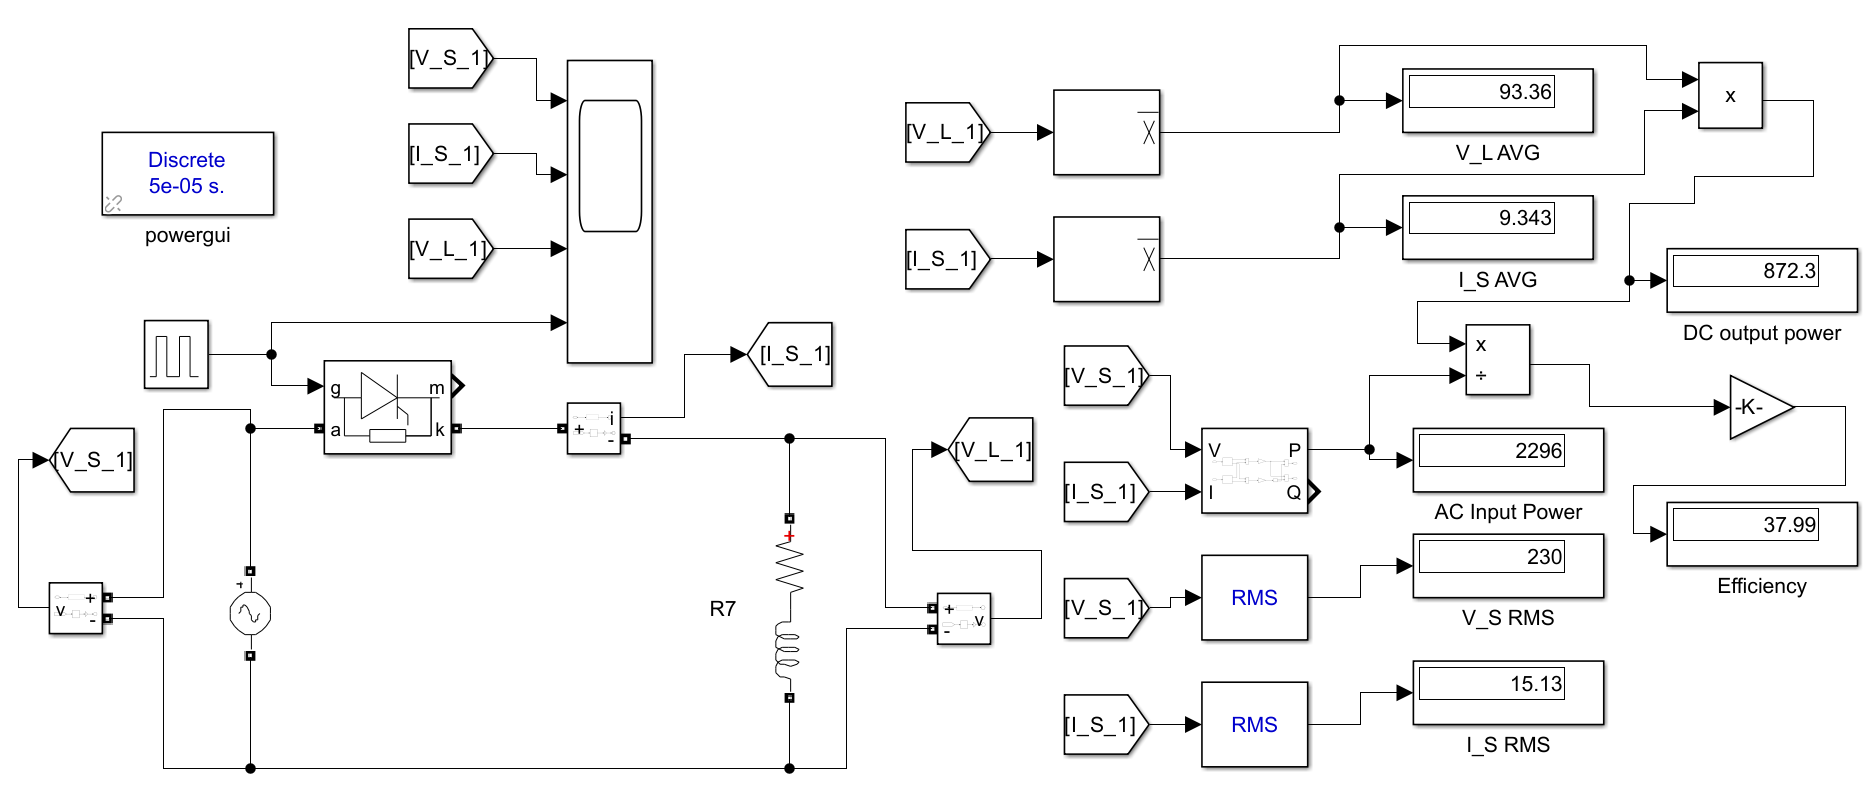
\includegraphics[width=1.0\textwidth]{images/experiment-1/circuit-diagram-experiment-06.png}
    \caption{Circuit for Single Phase Half Wave Controlled Rectifier with RL load  (Firing Angle = 30$ ^\circ $)}
    \label{Fig_simulation_circuit_single-phase-half-wave-controlled-rectifier-with-RL-load}
\end{figure}

\subsection{Components Required}

\begin{table}[h]
    \renewcommand{\arraystretch}{1.3}
    \label{table_components_required_single-phase-half-wave-controlled-rectifier-with-RL-load}
    \centering
    \begin{tabular}{|c|c|c|c|}
        \hline
        Sr. No & Parameters                     & Ratings            & Quantity \\
        \hline
        \hline
        1      & AC Single Phase Voltage Source & 230V ($ V_{rms} $) & 1        \\
        \hline
        2      & Resistor                       & 10$ \Omega $       & 1        \\
        \hline
        3      & Inductor                       & 10mH               & 1        \\
        \hline
        4      & Diode                          & -                  & 1        \\
        \hline
        5      & Voltmeter                      & -                  & 2        \\
        \hline
        6      & Ammeter                        & -                  & 1        \\
        \hline
        7      & Thyristor                      & -                  & 1        \\
        \hline
    \end{tabular}
    \caption{Components for Single Phase Half Wave Controlled Rectifier with RL load}

\end{table}




\subsection{Observations}

\begin{table}[h]
    \renewcommand{\arraystretch}{1.3}
    \label{table_observation_single-phase-half-wave-controlled-rectifier-with-RL-load}
    \centering
    \begin{tabular}{|c|c|c|}
        \hline
        Parameters                              & Theoretical Values & Simulation Values \\
        \hline
        \hline
        AC Input Voltage ($ V_{in,rms} $)       & 230V               & 230V              \\
        \hline
        Output Average Voltage ($ V_{o,avg} $)  & 96.6V              & 93.36V            \\
        \hline
        Output Average Current ($ I_{o,avg}  $) & 9.66A              & 9.343A            \\
        \hline
        AC Input Power ($ P_{AC}  $)            & 2214.44 (W)        & 2296 (W)          \\
        \hline
        DC Input Power ($ P_{DC}  $)            & 926.98 (W)         & 872.3 (W)         \\
        \hline
        Efficiency (\%)                         & 41.86              & 37.99             \\
        \hline
    \end{tabular}
    \caption{Observations for Single Phase Half Wave Controlled Rectifier with RL load}

\end{table}


It is observed that the circuit acts like an uncontrolled half wave rectifier only after the thyristor is triggered by a firing gate pulse. The output voltage waveform follows the shape of the RLE load waveform, and the output current lags the output voltage due to the inductive component of the load.
The efficiency of controlled rectifier with RL load is 37.99\%.


% \pagebreak

\subsection{Resultant Waveforms}

% figure that is centered on the page
\begin{figure}[h]
    \centering
    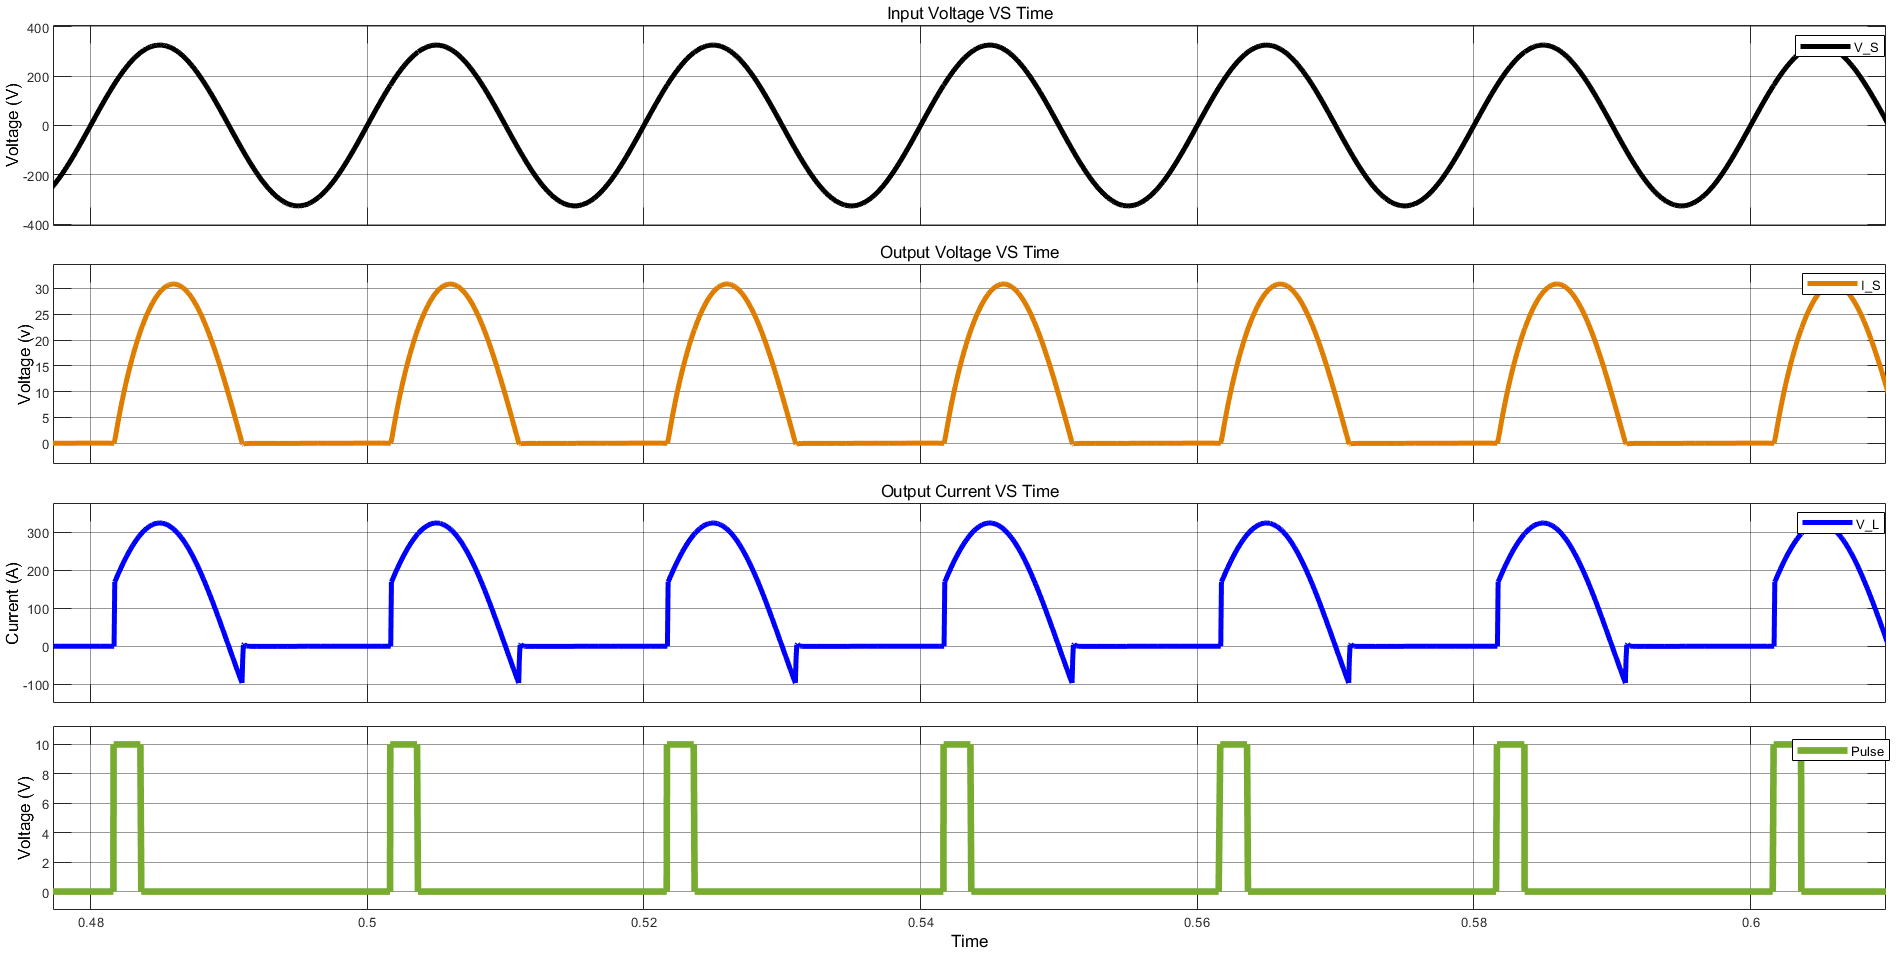
\includegraphics[width=1\textwidth]{images/experiment-1/circuit-scope-experiment-06.png}
    \caption{Scope Waveforms for Single Phase Half Wave Controlled Rectifier with RL load}
    \label{Fig_waveform_single-phase-half-wave-controlled-rectifier-with-RL-load}
\end{figure}

\pagebreak

%-----------------------circuit 2--------------------------
\section{Single Phase Half Wave Controlled Rectifier with RLE load}

\subsection{Circuit used for simulation}

% figure that is centered on the page
\begin{figure}[h]
    \centering
    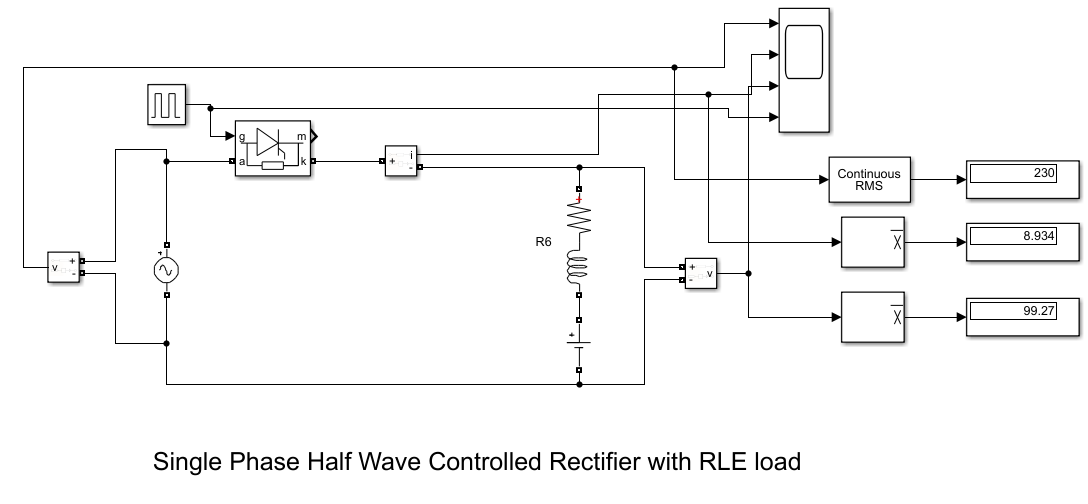
\includegraphics[width=0.7\textwidth]{images/experiment-1/circuit-diagram-simulation-07.png}
    \caption{Circuit used for simulation}
    \label{Fig_simulation_circuit_single-phase-half-wave-controlled-rectifier-with-RLE-load}
\end{figure}

\subsection{Components Required}

\begin{table}[h]
    \renewcommand{\arraystretch}{1.3}
    \label{table_components_required_circuit_7}
    \centering
    \begin{tabular}{|c|c|c|c|}
        \hline
        Sr. No & Parameters                     & Ratings            & Quantity \\
        \hline
        \hline
        1      & AC Single Phase Voltage Source & 230V ($ V_{rms} $) & 1        \\
        \hline
        2      & Resistor                       & 10$ \Omega $       & 1        \\
        \hline
        3      & Inductor                       & 10mH               & 1        \\
        \hline
        4      & Diode                          & -                  & 1        \\
        \hline
        5      & Voltmeter                      & -                  & 2        \\
        \hline
        6      & Ammeter                        & -                  & 1        \\
        \hline
        7      & Thyristor                      & -                  & 1        \\
        \hline
        8      & DC Source                      & 100V               & 1        \\
        \hline
    \end{tabular}
    \caption{Components for Single Phase Half Wave Controlled Rectifier with RLE load}

\end{table}

\pagebreak

\subsection{Observations}

\begin{table}[h]
    \renewcommand{\arraystretch}{1.3}
    \label{table_observation_7}
    \centering
    \begin{tabular}{|c|c|c|}
        \hline
        Parameters                              & Theoretical Values & Simulation Values \\
        \hline
        \hline
        AC Input Voltage ($ V_{in,rms} $)       & 230V               & 230V              \\
        \hline
        Output Average Voltage ($ V_{o,avg} $)  & 96.66V             & 154.8V            \\
        \hline
        Output Average Current ($ I_{o,avg}  $) & 9.66A              & 5.483A            \\
        \hline
        AC Input Power ($ P_{AC}  $)            & 2214.44 (W)        & 1459 (W)          \\
        \hline
        DC Input Power ($ P_{DC}  $)            & 926.98 (W)         & 848.6 (W)         \\
        \hline
        Efficiency (\%)                         & 41.86              & 58.18             \\
        \hline
    \end{tabular}
    \caption{Observations for Single Phase Half Wave Controlled Rectifier with RLE load}

\end{table}


Upon giving the firing gate pulse to the thyristor, the circuit is observed to initiate conduction. Once the circuit initiates conduction, its characteristics resemble those of an uncontrolled half wave rectifier with RLE load.
The efficiency of controlled rectifier with RL load is 58.18\%.



% \pagebreak


\subsection{Resultant Waveforms}

% figure that is centered on the page
\begin{figure}[h]
    \centering
    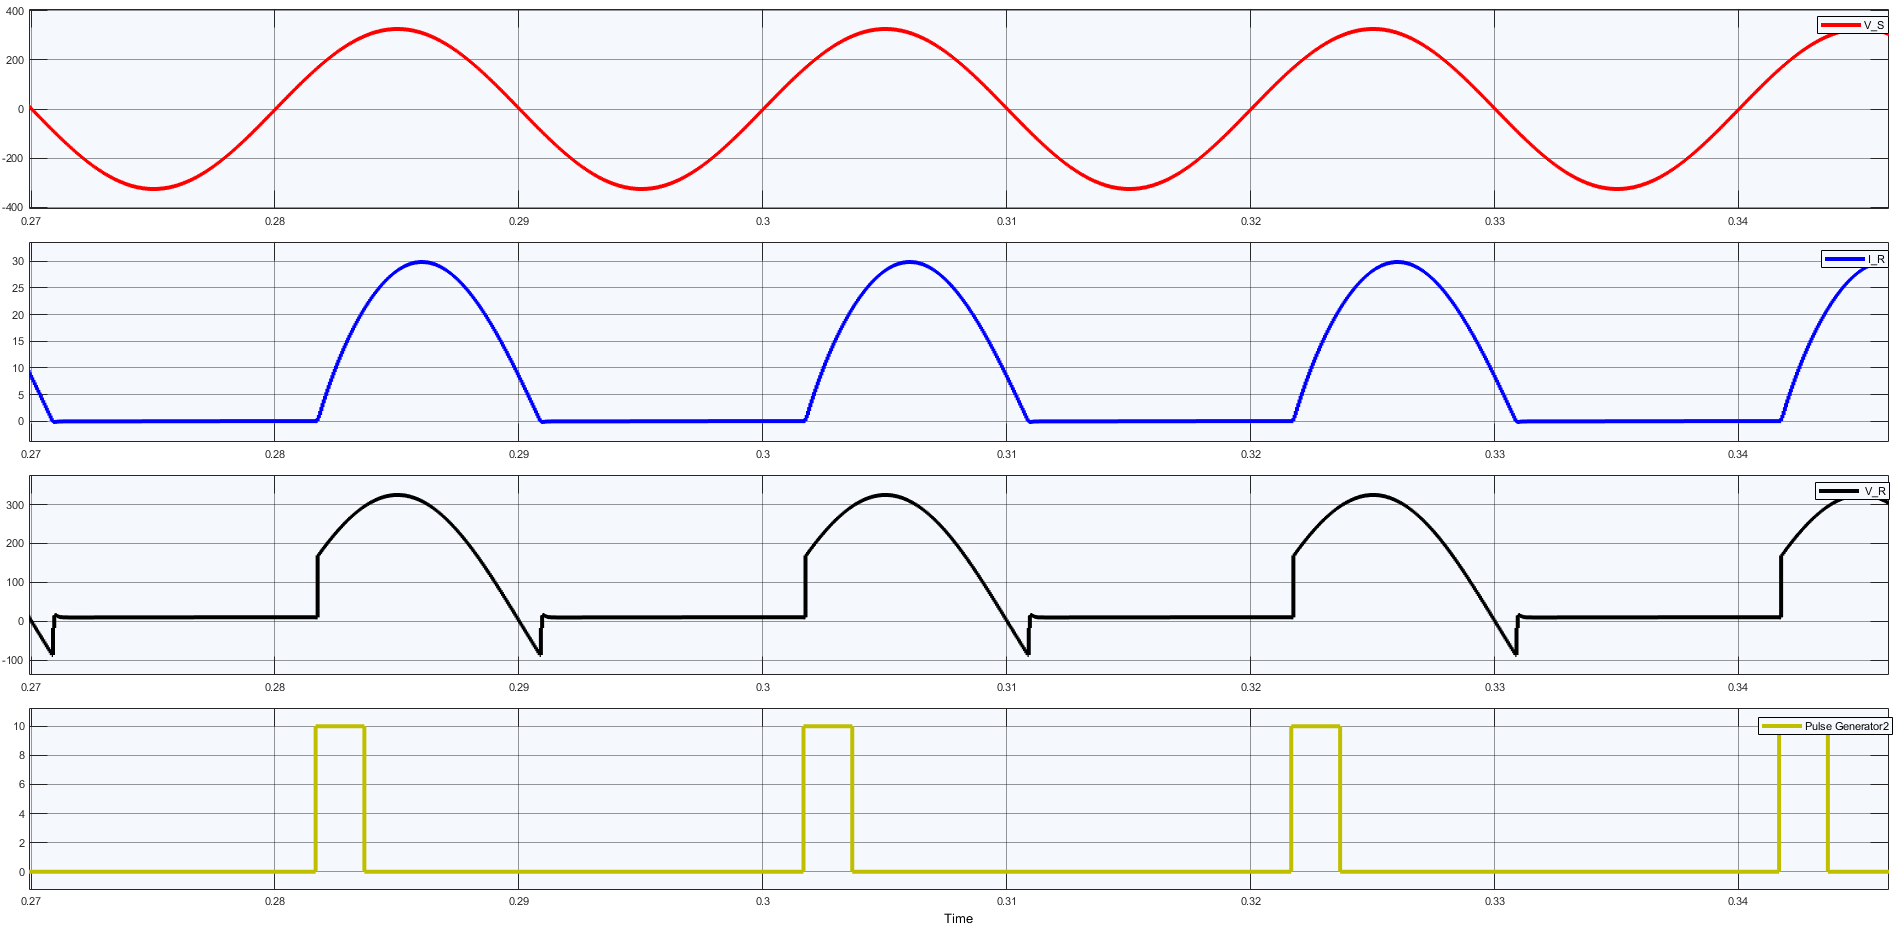
\includegraphics[width=1\textwidth]{images/experiment-1/circuit-scope-simulation-07.png}
    \caption{Scope Waveforms for Single Phase Half Wave Controlled Rectifier with RLE load}
    \label{Fig_waveform_single-phase-half-wave-controlled-rectifier-with-RLE-load}
\end{figure}


\pagebreak





\section{Conclusion}


\hspace{\parindent}

In this experiment, the implementation of single-phase half-wave rectifiers, both controlled and uncontrolled, with resistive, inductive, resistive-inductive and resistive-inductive with freewheeling diode loads were successfully accomplished using MATLAB's Simulink. The output waveforms for voltage and current were obtained in each case, and a comparative analysis between theoretically calculated and simulated output parameters was also performed.

Efficiency measurements were conducted on the half-wave uncontrolled rectifiers with R load, RL load, RL load with freewheeling diode, and RLE load, yielding efficiency values of 44.84\%, 43.84\%, 44.8\%, and 67.88\%, respectively. Thus, it can be concluded that the half-wave uncontrolled rectifier with RLE load has the maximum efficiency of 67.88\%. Similarly, the efficiency values of half-wave controlled rectifiers with R load, RL load, and RLE load were measured as 41.86\%, 40.85\%, 44.8\%, and 67.43\%, respectively. Thus, the half-wave controlled rectifier with RLE load has the maximum efficiency of 67.43\%.

Overall, the simulation results provided a clear indication of the efficiency of each type of rectifier with different loads. These results can be used as a guide to select the appropriate type of rectifier for a specific load in real-world applications. The implementation of these rectifiers has great practical significance in power electronics and can be used in a variety of applications, such as power supplies, motor drives, and lighting systems.
\pagebreak
